% !TEX encoding = UTF-8 Unicode
%!TEX root = thesis.tex
% !TEX spellcheck = en-US
%%=========================================
\chapter{Interface between Simulator and Control System}
This chapter will aim to decide an overall layout of the interface between the HIL Simulator and the control system to be tested. It will also be suggested an overview of the information flow between important modules of the simulator. Only a general layout will be suggested as the primary simulation target (Odin) is still under development and many details about the HW and SW solutions on board the boat are yet to be decided.

\newpage
\section{Overview of the Simulation Setup}
\begin{wrapfigure}[20]{r}{0.6\textwidth}
	\vspace{-45pt}
	\begin{center}
		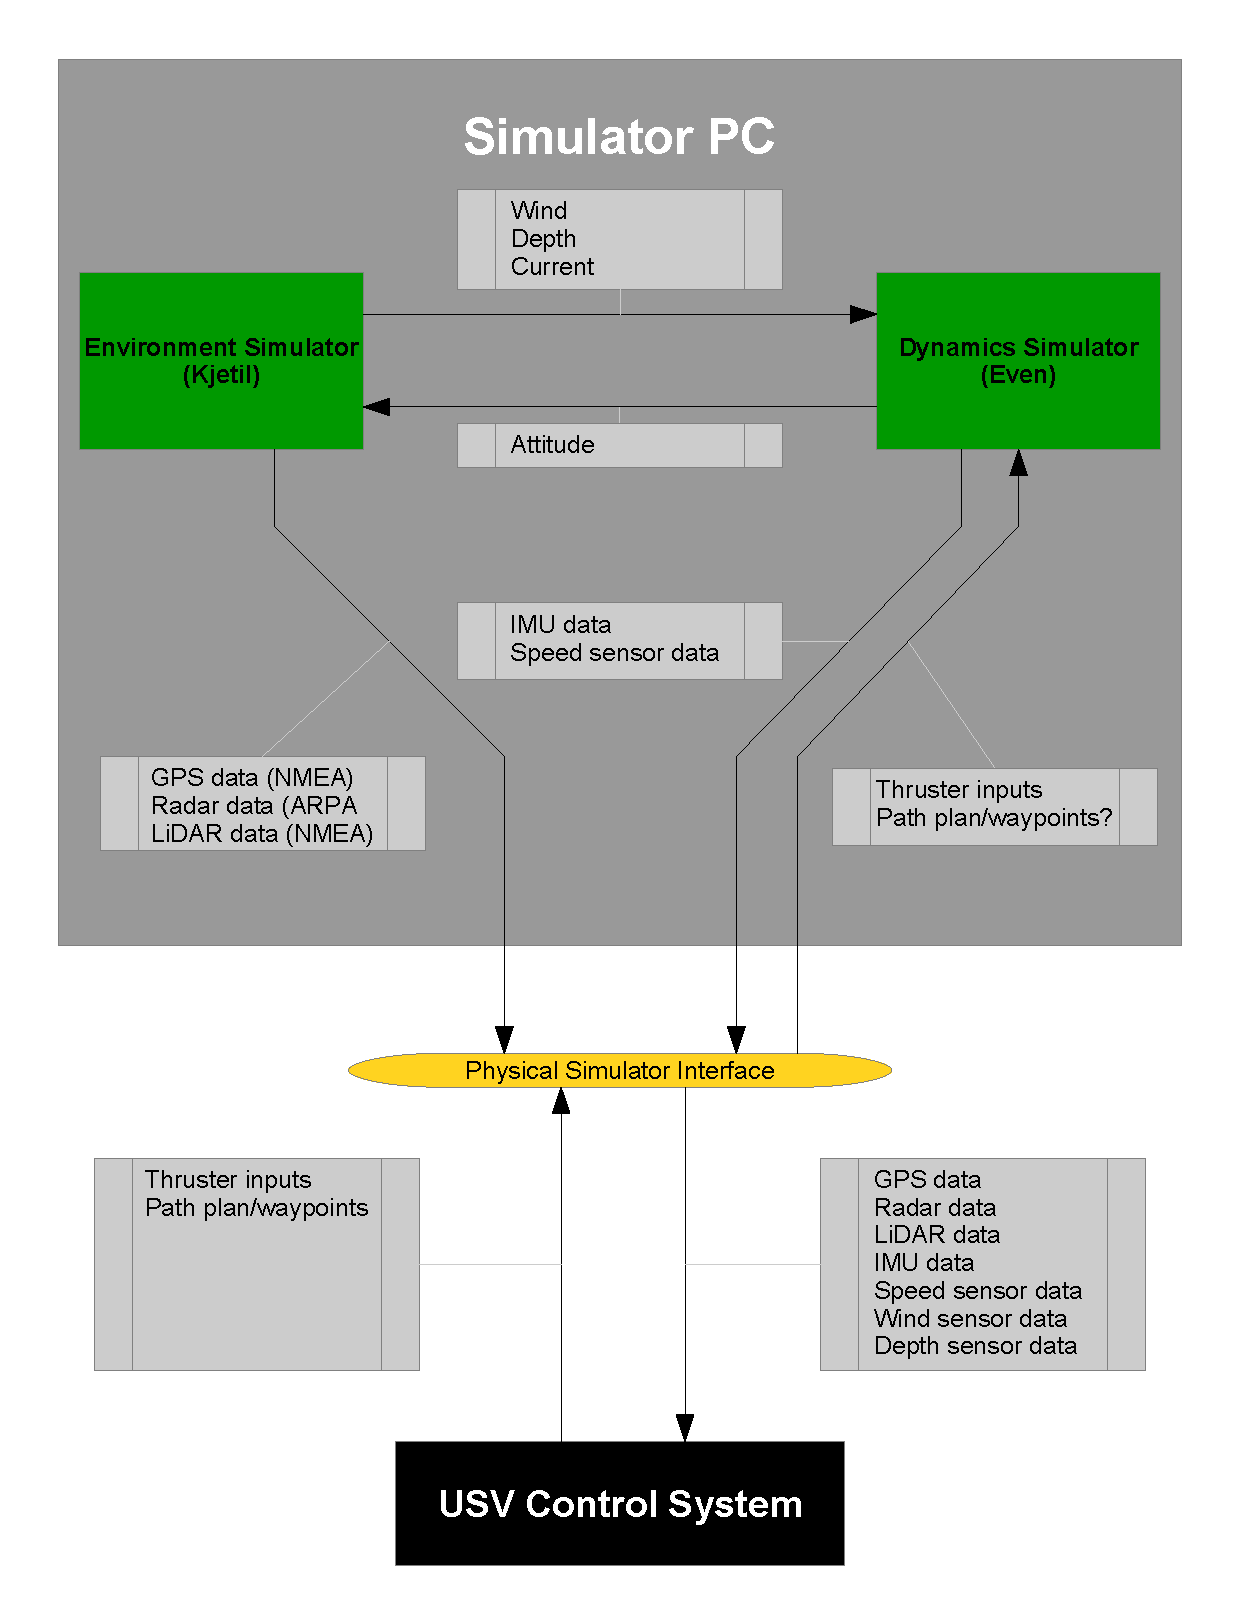
\includegraphics[width= 1\linewidth]{fig/Interface.pdf}
		\vspace{-40pt}
		\caption{\it{Simrad Broadband 4G radar used on Odin.}}
		\label{}
	\end{center}	
\end{wrapfigure}

The HIL Simulator should be run on a single laptop. The operating system (OS) should be Ubuntu to be able to utilize ROS functionality during simulation. The functionality of the simulator can The task of developing the simulator is divided in two project- and master thesis's: one for the simulation of 

\subsection{Message Protocol}


\section{Physical Interface}
Too early to decide the details of this.

